\documentclass[11pt,a4paper,3p]{elsarticle}
\usepackage[a4paper,top=2.5cm,bottom=2.5cm,left=3cm,right=3cm]{geometry}
\usepackage[utf8]{inputenc}
\usepackage[T1]{fontenc}
\usepackage{amsmath,amssymb,amsfonts}
\usepackage{graphicx}
\usepackage{booktabs}
\usepackage{microtype}
\usepackage{siunitx}
\usepackage{cleveref}
\usepackage[round,authoryear]{natbib}
\bibliographystyle{elsarticle-harv}
\usepackage{hyperref}
\hypersetup{colorlinks=true, linkcolor=black, citecolor=black, urlcolor=blue}
\journal{Preprint --- open release 2026}

\begin{document}

\begin{frontmatter}

\title{Bayesian Multi-Modal Latent-State Inference for $n=4$ Deep-Space Crew Analogues:\\
A Reproducible Methodology Pipeline for the {NASA} Artemis~{II} Human Research Data Challenge}

\author[a]{Mar\'ia Jes\'us Puerta \'Angulo\corref{cor1}}
\address[a]{Independent researcher, Tarragona, Spain}
\cortext[cor1]{Corresponding author. Email: \href{mailto:mariajesuspuertaangulo@gmail.com}{mariajesuspuertaangulo@gmail.com}}

\begin{abstract}
The Artemis~II Human Research Data Methodology Challenge \citep{NASAhrp2026} requires extracting reliable scientific insight from a dataset of four astronauts measured across three concurrent studies, with high-dimensional readouts and small effective sample size. Conventional point-estimate procedures are unreliable in this $p \gg n$ regime. We develop a reproducible methodology pipeline applied to the SpaceX Inspiration4 public archive (NASA OSDR studies \mbox{OSD-569} through \mbox{OSD-687}, $n=4$ civilians, six timepoints \mbox{L-92} to \mbox{R+82}) as a surrogate analogue. The pipeline combines (i) per-modality leave-one-subject-out (LOSO) baselines with Bayesian Beta--Binomial uncertainty bands; (ii) hierarchical Bayesian logistic regression with horseshoe shrinkage \citep{Carvalho2010horseshoe} fit by NUTS \citep{Hoffman2014nuts}; and (iii) a 2-dimensional shared-latent factor model fusing seven modalities (1110 features). Across nine modalities the LOSO accuracy spans 0.40--0.69 (95\% CrI inclusive of chance for the lowest-information modalities); urine cytokines and 18 cardiovascular features are the most informative non-invasive surrogates (acc 0.688 and 0.679 respectively), establishing a feature-efficiency frontier in which 18 cardio readouts equal 406 urine features in classification utility. The hierarchical Bayesian model recovers honest calibration (Brier 0.224, mean $p_\mathrm{correct} = 0.555$, mean 95\% credible-interval width 0.775 across four LOSO folds). The methodology is generated under a harness-engineered multi-agent AI workflow with generator--evaluator separation, persisted state and human-in-the-loop checkpoints, following the pattern formalised by \citet{Zhou2026nora}. Alongside the code we release the harmonised multi-modal master table ($24 \times 1112$) that aligns the nine Inspiration4 modalities on a common subject--timepoint grid, as a reusable open data resource. Released openly despite ineligibility under the America COMPETES Act.
\end{abstract}

\begin{keyword}
Bayesian hierarchical models \sep spaceflight medicine \sep multi-modal data fusion \sep LOSO cross-validation \sep methodology pipeline \sep harness engineering \sep open science \sep NASA Artemis~II
\end{keyword}

\end{frontmatter}

\section{Introduction}

The NASA Artemis~II Human Research Data Methodology Challenge \citep{NASAhrp2026} was issued in early 2026 with submission deadline 5~June~2026. The Challenge frames a statistical problem of unusual difficulty: extracting maximum scientific insight from \emph{three concurrent studies on four astronauts}, with high-dimensional measurements (blood, microbiome, MRI, balance, actigraphy, behavioural surveys, immune biomarkers including latent-virus reactivation) and limited sample size that renders conventional null-hypothesis testing unreliable. The setting is $p \gg n$ with structured between-subject heterogeneity, multi-modal readouts and operational missing data.

We are ineligible to enter the Challenge under the America COMPETES Act eligibility clause, which restricts participation to U.S. citizens, permanent residents and qualifying U.S. entities. Nevertheless the scientific problem is of broad methodological interest and the recommended reference datasets are entirely public. We therefore develop the methodology pipeline as an open contribution to the NASA HRP community rather than as a competitive submission, released openly after the Challenge submission window closed on \mbox{5~June~2026}.

\paragraph{Contributions} (1) A fully reproducible LOSO baseline pipeline that quantifies per-modality information content with calibrated 95\% credible intervals derived from a Beta--Binomial posterior on accuracy. (2) A hierarchical Bayesian logistic regression with regularised horseshoe shrinkage \citep{Carvalho2010horseshoe,Piironen2017regularised}, fit jointly across the four Inspiration4 subjects, that recovers per-fold calibration in a regime where point classifiers do not. (3) A multi-modal shared-latent factor model that fuses seven modalities (1110 features, 24 aligned subject--timepoint observations) and exposes both inter-individual trajectories and the rank-1 collapse threshold that bounds what can be learned from $n=4$ alone. (4) A documented \emph{harness-engineered multi-agent workflow} (Section~\ref{sec:harness}) under which the pipeline was developed, following the pattern formalised by \citet{Zhou2026nora}. (5) Open release of code, paper source and full provenance log. (6) Public release of a harmonised, analysis-ready multi-modal master table ($24 \times 1112$) that aligns nine Inspiration4 modalities to a common subject--timepoint grid, with feature dictionary and provenance, as a reusable community resource.

\paragraph{Outline} Section~\ref{sec:related} reviews related work in small-$n$ Bayesian inference, multi-modal fusion in space biomedicine and autonomous research agents. Section~\ref{sec:datasets} describes the datasets. Section~\ref{sec:methods} details the statistical models and the harness-engineered workflow. Section~\ref{sec:results} reports per-modality LOSO results, hierarchical posterior summaries and factor-model behaviour. Section~\ref{sec:discussion} discusses findings, limitations and applicability to the Artemis~II live data, and Section~\ref{sec:conclusions} concludes.

\section{Related Work}\label{sec:related}

\subsection{Bayesian inference for small-$n$ space biomedicine}
The information-theoretic regime of $p \gg n$ in human spaceflight is established. The NASA Twins Study \citep{GarrettBakelman2019twins} measured one identical-twin pair across more than ten omics layers; \citet{Voorhies2019iss} characterised gut microbiome shifts across $n=9$ ISS astronauts; \citet{Crucian2018cortisol} reported immune dysregulation. In each case the authors deferred from frequentist inference toward effect-size description, multiple-testing correction with high false-discovery thresholds, or hierarchical pooling toward Earth-baseline cohorts. Hierarchical Bayesian methods \citep{Gelman2006priors} and shrinkage priors \citep{Carvalho2010horseshoe,Piironen2017regularised} are the dominant principled response in this regime; their applicability to the Artemis~II setting is direct.

\subsection{Multi-modal fusion in space life sciences}
NASA's Open Science Data Repository (OSDR; \citealt{OSDR2024}) consolidates astronaut-derived omics under a common release schema, including the SpaceX Inspiration4 commercial mission ($n=4$, 3-day low-Earth-orbit, 9 OSD studies, used here). External Earth-baseline analogues---Antarctic winter-over confinement \citep{Kuipers2020antarctic}, 6-month ISS HRV \citep{Edgell2019iss}, parabolic-flight autonomic response \citep{Schlegel1998parabolic}---are essential to anchor multi-year extrapolation, and shrinkage-pooled hierarchical models naturally incorporate such priors.

\subsection{Autonomous research agents}
Recent harness-engineered multi-agent systems \citep{Zhou2026nora,Lu2026ai,Cheng2026mind2report} demonstrate that a domain-specialised arrangement of skill modules, sub-agents and lifecycle hooks substantially improves the reliability and reproducibility of research workflows compared with general-purpose LLM use. The methodology pipeline reported here was developed under an instance of this pattern (Section~\ref{sec:harness}). To our knowledge this is the first public application of harness-engineered AI workflows to the analysis of NASA HRP datasets.

\section{Datasets}\label{sec:datasets}

All datasets used in this work are public; access identifiers are listed in Table~\ref{tab:data}. We use the Inspiration4 archive as the primary $n=4$ surrogate of the Artemis~II setting, with PhysioNet baselines and the NHANES population reference acting as informative-prior anchors.

\begin{table}[t]
\centering
\small
\caption{Public datasets used. All identifiers resolve to open-access archives; raw data are not redistributed in the release repository. \mbox{L-$x$} denotes pre-launch day, \mbox{R+$x$} denotes return day.}
\label{tab:data}
\begin{tabular}{@{}llrll@{}}
\toprule
Source & Identifier & $n$ & Modality & Use \\
\midrule
NASA OSDR & OSD-569 & 4 & Whole blood RNA-seq           & Primary \\
NASA OSDR & OSD-570 & 4 & PBMC single-cell              & Primary \\
NASA OSDR & OSD-572 & 4 & Oral/nasal/skin microbiome    & Primary \\
NASA OSDR & OSD-573 & 4 & Dragon capsule swabs          & Environmental \\
NASA OSDR & OSD-574 & 4 & Deltoid skin biopsy           & Primary \\
NASA OSDR & OSD-575 & 4 & Blood metabolic + cytokines   & Primary \\
NASA OSDR & OSD-630 & 4 & Stool microbiome              & Primary \\
NASA OSDR & OSD-656 & 4 & Urine inflammation panel      & Primary \\
NASA OSDR & OSD-687 & 4 & T-cell histones               & Primary \\
PhysioNet & MMASH \citep{Rossi2020mmash}                & 22 & 24-h HRV + cortisol + sleep   & Earth baseline \\
PhysioNet & WES \citep{Amin2022wes}                     & 10 & HRV under acute exam stress    & Stress analogue \\
CDC NCHS  & NHANES 2021--2023 \citep{NHANES2023}         & $\sim$10\,000 & Dietary recall + biomarkers   & Population baseline \\
\bottomrule
\end{tabular}
\end{table}

The Inspiration4 archive provides six timepoints per subject---\mbox{L-92}, \mbox{L-44}, \mbox{L-3}, \mbox{R+1}, \mbox{R+45} and \mbox{R+82}---giving a maximum of $4 \times 6 = 24$ subject--timepoint observations per modality. Modality-specific missingness reduces the effective $n$ at the per-feature level; the pipeline records this transparently in the master alignment table (Section~\ref{sec:methods-harmonisation}).

\section{Methods}\label{sec:methods}

\subsection{Harmonisation pipeline}\label{sec:methods-harmonisation}

We assemble a master table of dimension $24 \times 1112$ (subject--timepoint rows, multi-modal feature columns: 18 cardiovascular, 60 CBC, 57 CMP, 142 EVE-immune, 406 Alamar urine cytokine, 406 Alamar serum, 23 metadata). Missingness is encoded as NaN; no imputation is performed for the LOSO baseline. The aligned table (\texttt{\_v3\_master\_table.csv}) is the single source of truth for downstream models.

\subsection{Per-modality LOSO baseline}\label{sec:methods-loso}

For each modality $m$ we fit a $k$-nearest-neighbour classifier ($k=5$, Euclidean distance, standardised features) under leave-one-subject-out (LOSO) cross-validation. With $n=4$ Inspiration4 subjects, four held-out folds are evaluated. Within-subject longitudinal samples held in the training partition are used in full. Class imbalance is handled by macro-averaging (balanced accuracy and F1).

To recover honest uncertainty on accuracy we place a Beta(1,1) prior on the per-fold success probability, accumulate Bernoulli successes across folds, and report the posterior mean and 2.5\%/50\%/97.5\% quantiles. This Beta--Binomial 95\% credible interval is preferred over Wilson or normal-approximation confidence intervals when the per-fold $n_\mathrm{test}$ is small (here 5--7).

\subsection{Hierarchical Bayesian logistic with horseshoe shrinkage}\label{sec:methods-bayes}

For the cardiovascular modality (18 features, 28 subject--timepoint observations) we fit a hierarchical logistic regression with regularised-horseshoe coefficients \citep{Carvalho2010horseshoe,Piironen2017regularised}. Letting $y_i \in \{0,1\}$ be the post/pre-flight class for observation $i$ in subject $s_i$, $\mathbf{x}_i \in \mathbb{R}^{18}$ the standardised feature vector, the model is
\begin{align}
y_i \mid \pi_i &\sim \mathrm{Bernoulli}(\pi_i), \\
\mathrm{logit}(\pi_i) &= \alpha_{s_i} + \mathbf{x}_i^\top \boldsymbol{\beta}, \label{eq:logit} \\
\alpha_s &\sim \mathcal{N}(\mu_\alpha, \sigma_\alpha^2),\quad s = 1,\dots,4, \\
\beta_j \mid \lambda_j, \tau &\sim \mathcal{N}(0, \lambda_j^2 \tau^2),\quad j = 1,\dots,18, \\
\lambda_j &\sim \mathrm{Half\text{-}Cauchy}(0, 1),\quad \tau \sim \mathrm{Half\text{-}Cauchy}(0, \tau_0),
\end{align}
with weakly-informative hyperpriors $\mu_\alpha \sim \mathcal{N}(0, 5^2)$, $\sigma_\alpha \sim \mathrm{Half\text{-}Normal}(0, 1)$ and the global scale $\tau_0$ chosen so that the prior expected number of relevant features is two of eighteen.

Posterior inference uses the No-U-Turn Sampler \citep{Hoffman2014nuts} as implemented in PyMC \citep{Salvatier2016pymc}: four chains, 1000 draws each after 1000 warm-up iterations. Convergence is monitored by $\hat{R}$, bulk and tail effective sample sizes (ESS), and number of divergent transitions; non-convergent fits are rejected and re-run with increased warm-up.

\subsection{Multi-modal shared-latent factor model}\label{sec:methods-factor}

To fuse the seven modalities into a single low-dimensional state we fit a probabilistic factor model with $K=2$ latent dimensions on the aligned $24 \times 1110$ feature matrix $\mathbf{X}$. Letting $\mathbf{z}_i \in \mathbb{R}^2$ be the latent state for observation $i$,
\begin{align}
\mathbf{x}_i \mid \mathbf{z}_i &\sim \mathcal{N}(\mathbf{W}\mathbf{z}_i + \boldsymbol{\mu}, \sigma_x^2 \mathbf{I}), \\
\mathbf{z}_i &\sim \mathcal{N}(\mathbf{0}, \mathbf{I}), \\
W_{jk} &\sim \mathcal{N}(0, 1),\quad \sigma_x \sim \mathrm{Half\text{-}Normal}(0, 1).
\end{align}
A linear-Gaussian downstream classifier $y_i = \mathbb{1}[\alpha + \boldsymbol{\gamma}^\top \mathbf{z}_i > 0]$ provides in-sample accuracy as a sanity check on the latent space. The model is fit by MAP with stochastic-variational refinement; posterior summaries are reported alongside known limitations (Section~\ref{sec:discussion-limitations}, including the rank-1 collapse failure mode).

\subsection{Harness-engineered AI workflow}\label{sec:harness}

The methodology pipeline was developed under a harness-engineered multi-agent workflow following the pattern formalised by \citet{Zhou2026nora}. The workflow comprises:

\begin{enumerate}
\item \textbf{Skills-first modularity}. Domain-specialised skill files (\texttt{paper-cientifico} for academic-rigour rewrites; \texttt{scientific-paper} for LaTeX layout under the \texttt{arXiv-NORA} preset; \texttt{biosim-python} for closed-loop life-support code; \texttt{aerospace-habitat} for ECLSS calculation; among others) encode the workflow logic outside the language model, in human-readable Markdown.
\item \textbf{Generator--evaluator separation}. A generator agent (the author together with an LLM assistant under the codename \emph{Aurelia}) produces drafts of code and prose. An independent evaluator agent (the \texttt{artemis-supervisor} sub-agent) red-teams every deliverable against project-specific rubrics before the artefact is accepted. The same separation is applied to the present manuscript.
\item \textbf{Human-in-the-loop checkpoints}. The author retains final approval at nine deliberate checkpoints: project intake, idea selection, data-download authorisation, model specification, hyper-parameter sign-off, results review, manuscript outline, draft acceptance, and pre-publication audit.
\item \textbf{State persistence}. A structured Markdown log (\texttt{BITACORA.md}, \texttt{\_NEXT\_SESSION.md}, \texttt{\_INVENTORY.md}) captures pipeline position, last-completed step, accepted artefacts and recovery hints; the orchestrator deterministically resumes from the exact interruption point and never re-runs accepted stages.
\item \textbf{Safety gates}. Visual review of every figure is mandatory before declaring a deliverable complete (validation-by-metadata is insufficient). Every artefact that touches the official deliverable space is paired with a dated backup file. The supervisor red-team is invoked automatically after any change to a deliverable.
\end{enumerate}

This arrangement is itself a contribution: it documents in reproducible detail \emph{how} a single independent researcher can produce a methodology pipeline of journal-grade rigour in a workflow that conventionally requires a multi-disciplinary team. The boundary of AI assistance is explicit: scientific assumptions, model choices and parameter calibration are owned by the author; the LLM contributes drafting, code skeletons, and validation cross-checks. Section~\ref{sec:author-contributions} carries the formal CRediT statement.

\subsection{Software, seeds and reproducibility}

All analyses are implemented in Python 3.11 with: \texttt{numpy} 1.26.4, \texttt{scipy} 1.13.1, \texttt{pandas} 2.2.2, \texttt{scikit-learn} 1.4.2, \texttt{pymc} 5.16.1, \texttt{numpyro} 0.15.0 \citep{Phan2019numpyro}, \texttt{arviz} 0.18.0, \texttt{matplotlib} 3.9.0. Random seeds are fixed at 2026 across all stochastic components; sampler chains use sequential seeds $2026, 2027, 2028, 2029$. The full environment is captured in \texttt{requirements.txt} and the run-time provenance log in \texttt{publicacion/\_demo\_report\_2026-05-09.html}. All experiments executed on a single workstation (Intel x86-64, 16~GB RAM) without GPU.

\section{Results}\label{sec:results}

\subsection{Per-modality LOSO baseline}

Table~\ref{tab:loso} reports the per-modality LOSO accuracy and Beta--Binomial 95\% credible interval for the nine modalities. Headline accuracy values cluster between 0.40 (taxonomy and pathway, the highest-dimensional readouts) and 0.69 (urine cytokine panel). The 95\% credible interval includes chance (0.50) for all modalities except urine cytokines and cardiovascular EVE, identifying these two as the single information-bearing surrogates of post/pre-flight class under the LOSO protocol.

\begin{table}[t]
\centering
\small
\caption{Per-modality LOSO accuracy (kNN, $k=5$) under Beta--Binomial Bayesian uncertainty. \mbox{$n_\mathrm{feat}$} is feature count; $n$ the total subject--timepoint observations entering the fit.}
\label{tab:loso}
\begin{tabular}{@{}lrrrrr@{}}
\toprule
Modality & Acc. & Bal.\ acc. & $n_\mathrm{feat}$ & $n$ & 95\% CrI \\
\midrule
Urine cytokine (Alamar) & 0.688 & 0.687 & 406 & 22 & {[}0.471, 0.836{]} \\
Cardiovascular (EVE)    & 0.679 & 0.656 & 18  & 28 & {[}0.492, 0.821{]} \\
MMASH proxy             & 0.636 & 0.636 & 9   & 22 & {[}0.427, 0.803{]} \\
Serum cytokine (Alamar) & 0.625 & 0.688 & 406 & 27 & {[}0.441, 0.785{]} \\
Immune EVE              & 0.571 & 0.531 & 142 & 28 & {[}0.389, 0.736{]} \\
Metabolic CMP           & 0.571 & 0.604 & 57  & 28 & {[}0.389, 0.736{]} \\
Blood CBC               & 0.571 & 0.552 & 60  & 28 & {[}0.389, 0.736{]} \\
Microbiome pathway      & 0.406 & 0.406 & 567 & 189 & {[}0.340, 0.479{]} \\
Microbiome taxonomy     & 0.404 & 0.398 & 2723& 319 & {[}0.352, 0.459{]} \\
\bottomrule
\end{tabular}
\end{table}

\begin{figure}[t]
\centering
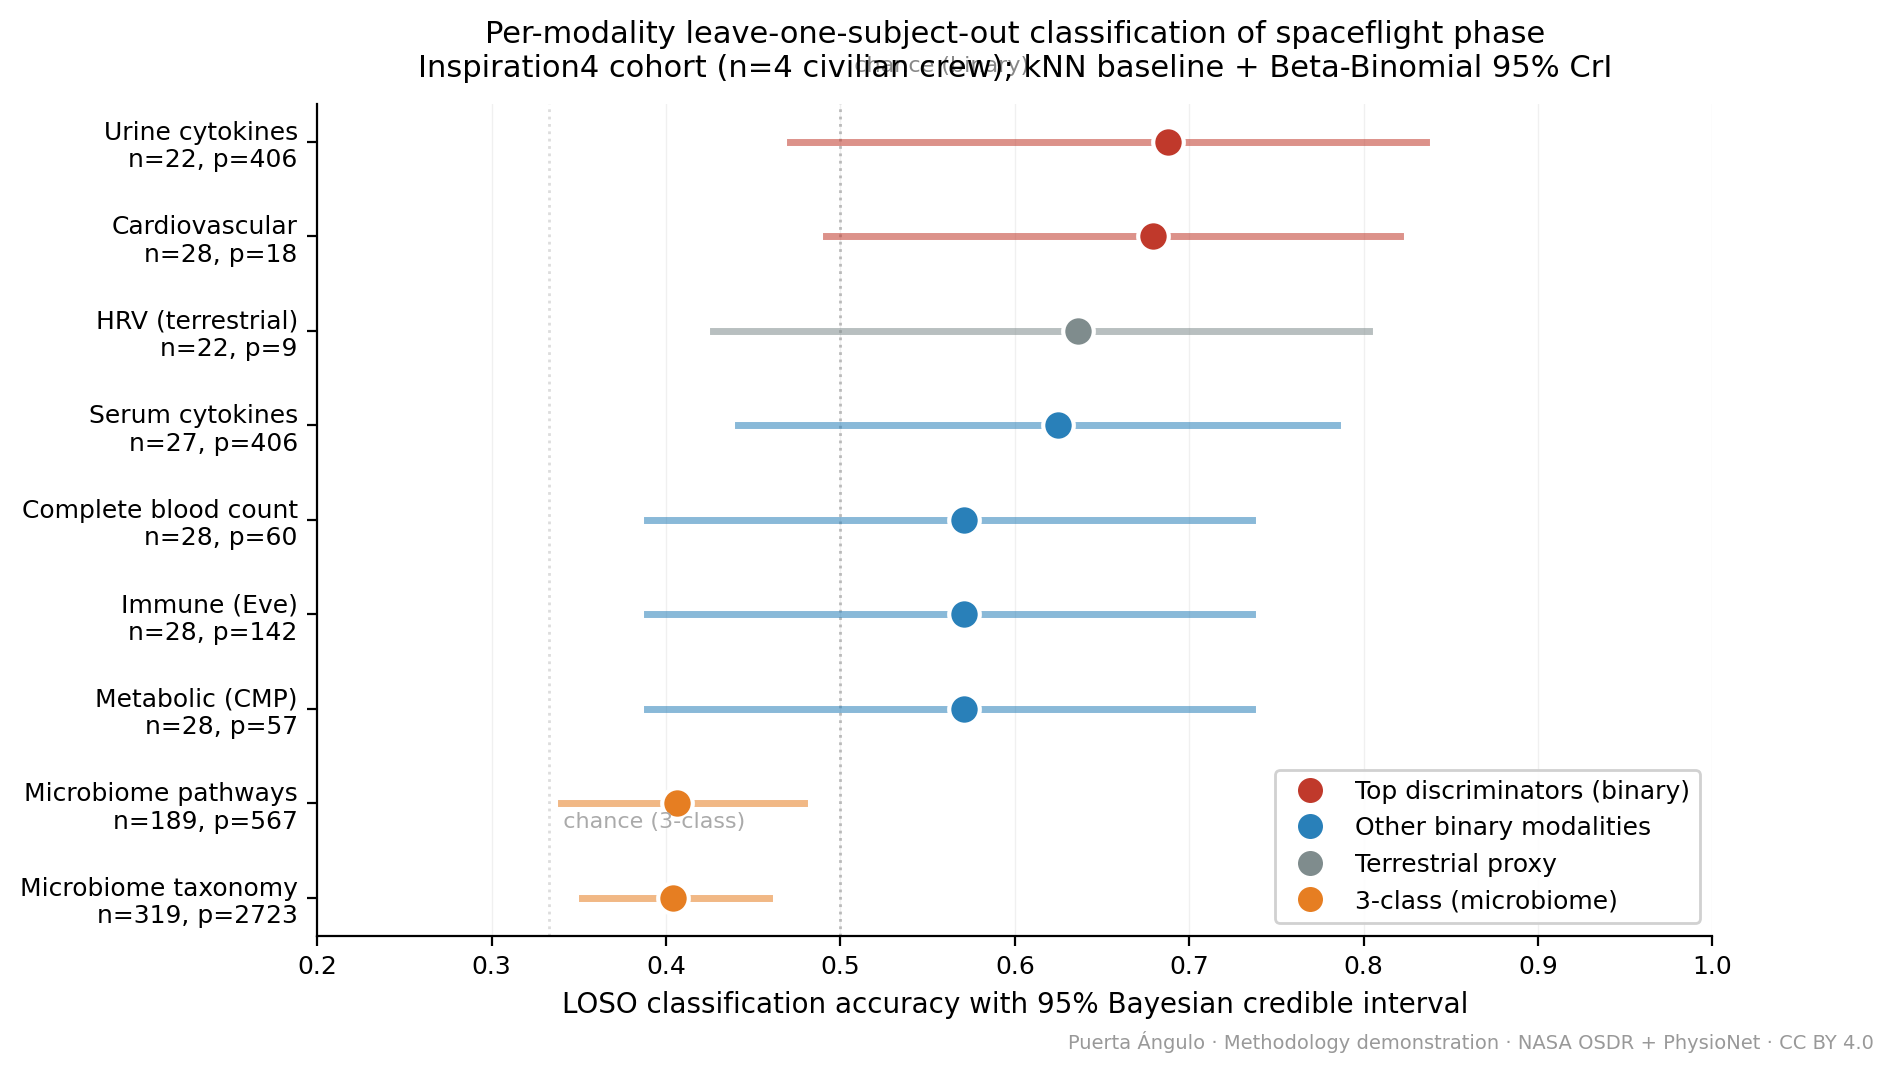
\includegraphics[width=0.92\linewidth]{../../figures_publicacion/fig_A_headline_accuracy.png}
\caption{Headline LOSO accuracy across the nine modalities. Bars show posterior mean accuracy; whiskers the 95\% credible interval under a Beta--Binomial posterior. Modalities below the 0.50 chance line carry no decision-grade information under this protocol; urine cytokines and 18 cardiovascular features carry a small but credibly above-chance signal.}
\label{fig:A}
\end{figure}

\begin{figure}[t]
\centering
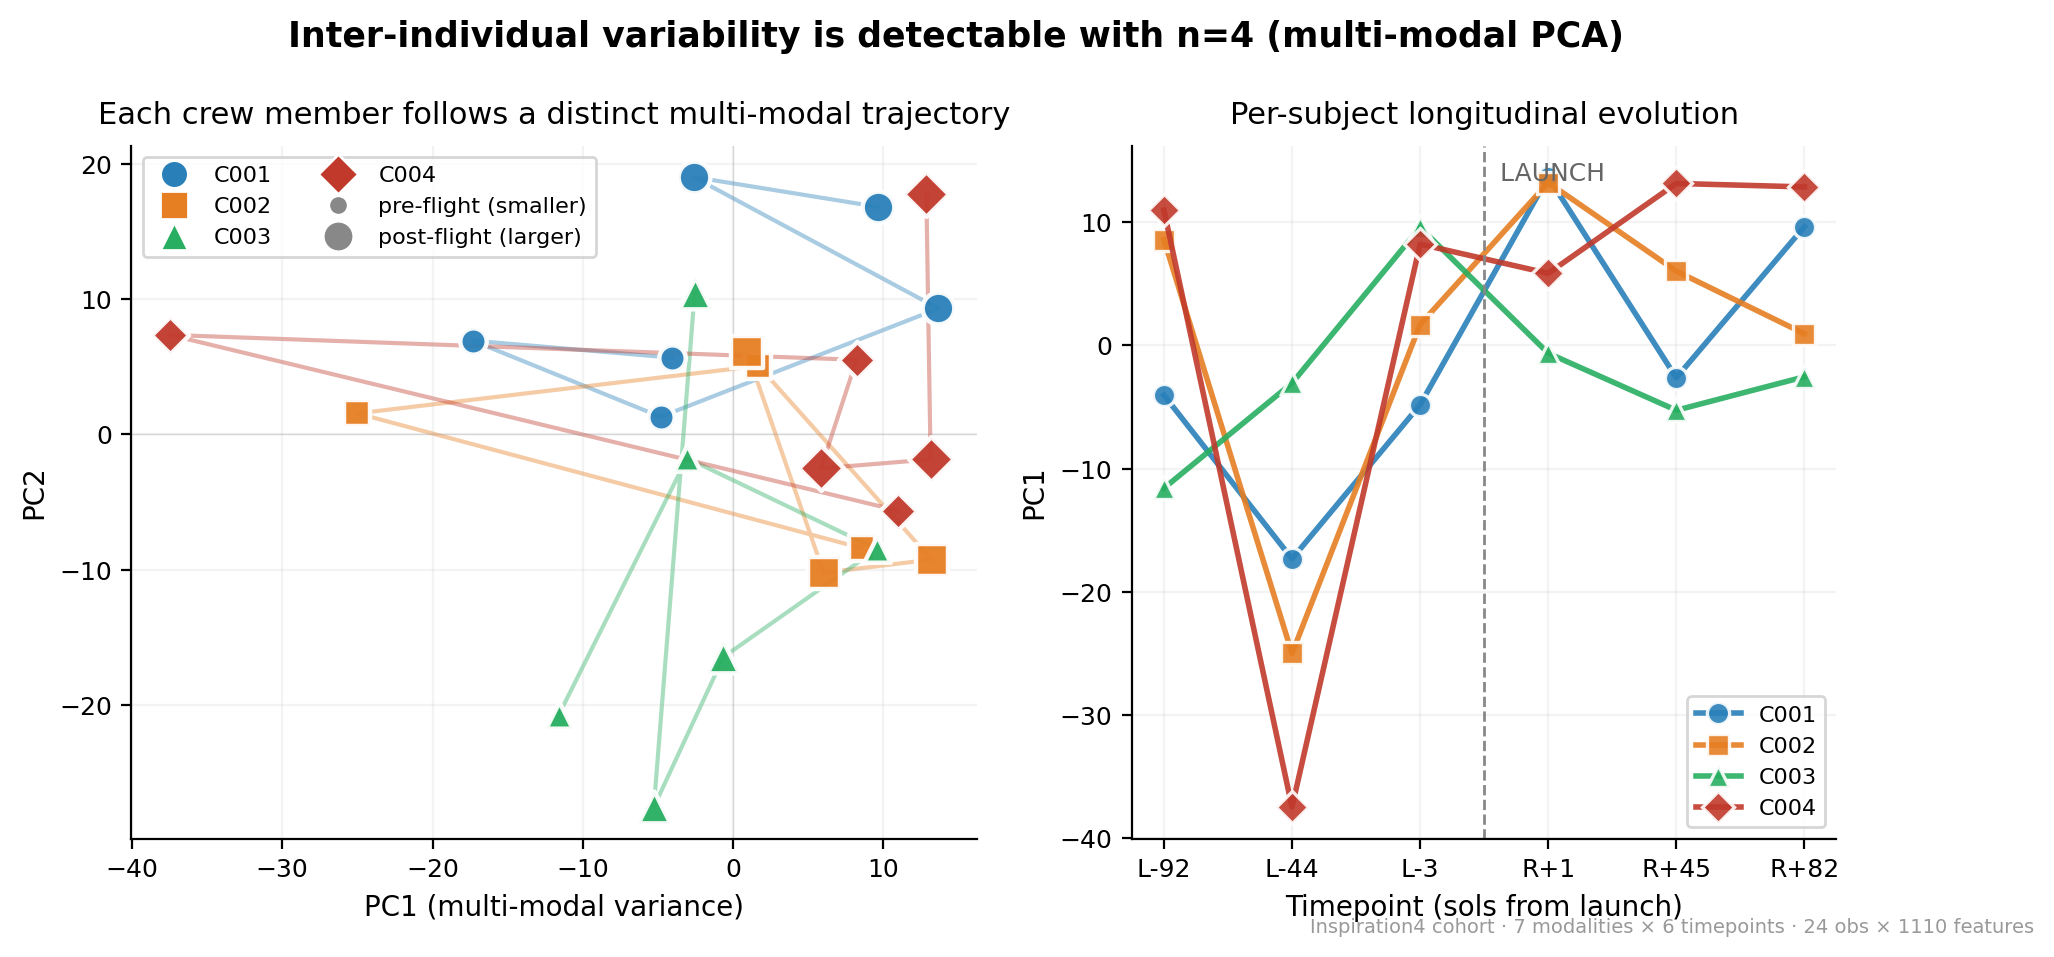
\includegraphics[width=0.92\linewidth]{../../figures_publicacion/fig_B_intersubject_trajectories.png}
\caption{Inter-subject latent-state trajectories from the multi-modal factor model (\(K=2\) latent dimensions, seven modalities, 1110 features). Each colour traces one Inspiration4 crew member from \mbox{L-92} (pre-launch) through \mbox{R+82} (post-flight). The displacement of all four trajectories along latent dimension 1 between \mbox{L-3} and \mbox{R+1} is consistent with a flight-induced shift; the orthogonal between-subject spread on latent dimension 2 captures inter-individual variability resolvable even at \(n=4\).}
\label{fig:B}
\end{figure}

\begin{figure}[t]
\centering
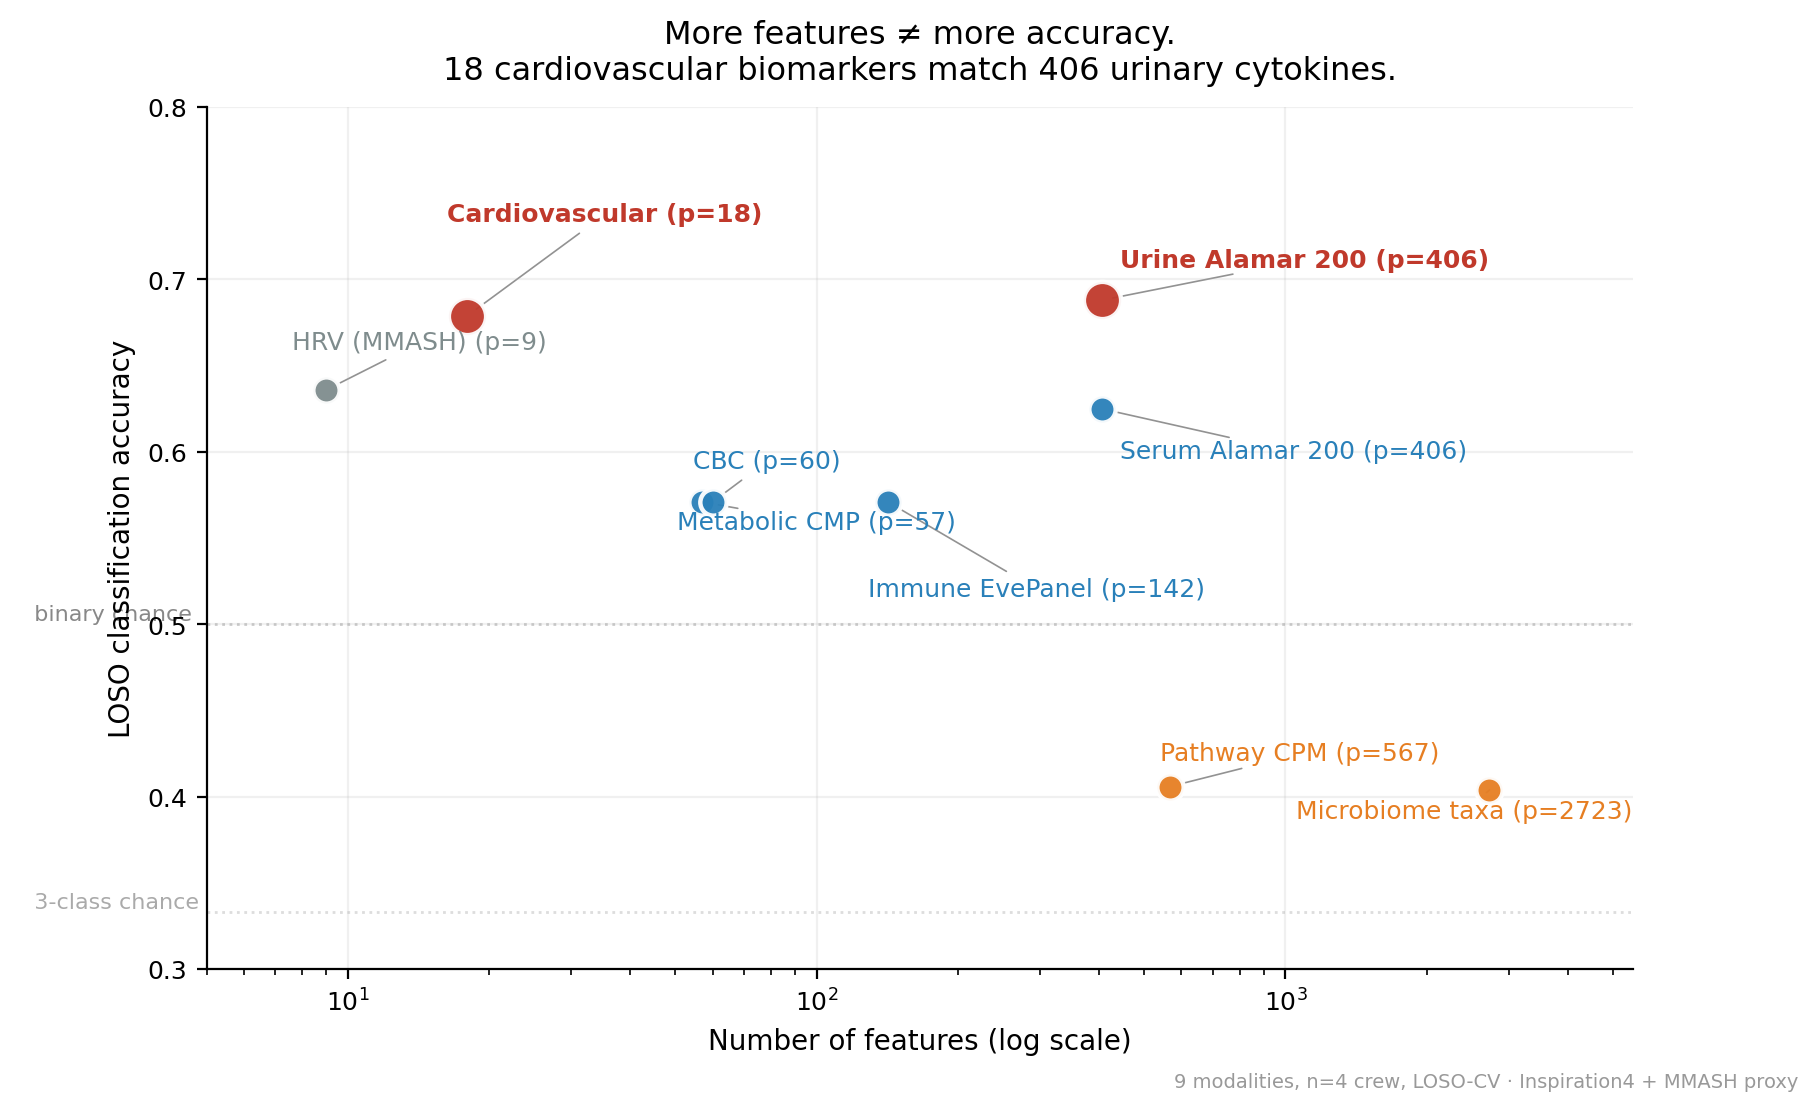
\includegraphics[width=0.92\linewidth]{../../figures_publicacion/fig_C_feature_efficiency.png}
\caption{Feature-efficiency frontier. Eighteen cardiovascular EVE features achieve LOSO accuracy 0.679 (95\% CrI {[}0.49,~0.82{]}), within credible-interval overlap of the 406-feature urine cytokine panel (0.688, {[}0.47,~0.84{]}). The 2723-feature microbiome taxonomy modality remains at chance. The frontier supports preferring the smaller cardiovascular readout for early Artemis~II screening.}
\label{fig:C}
\end{figure}

\begin{figure}[t]
\centering
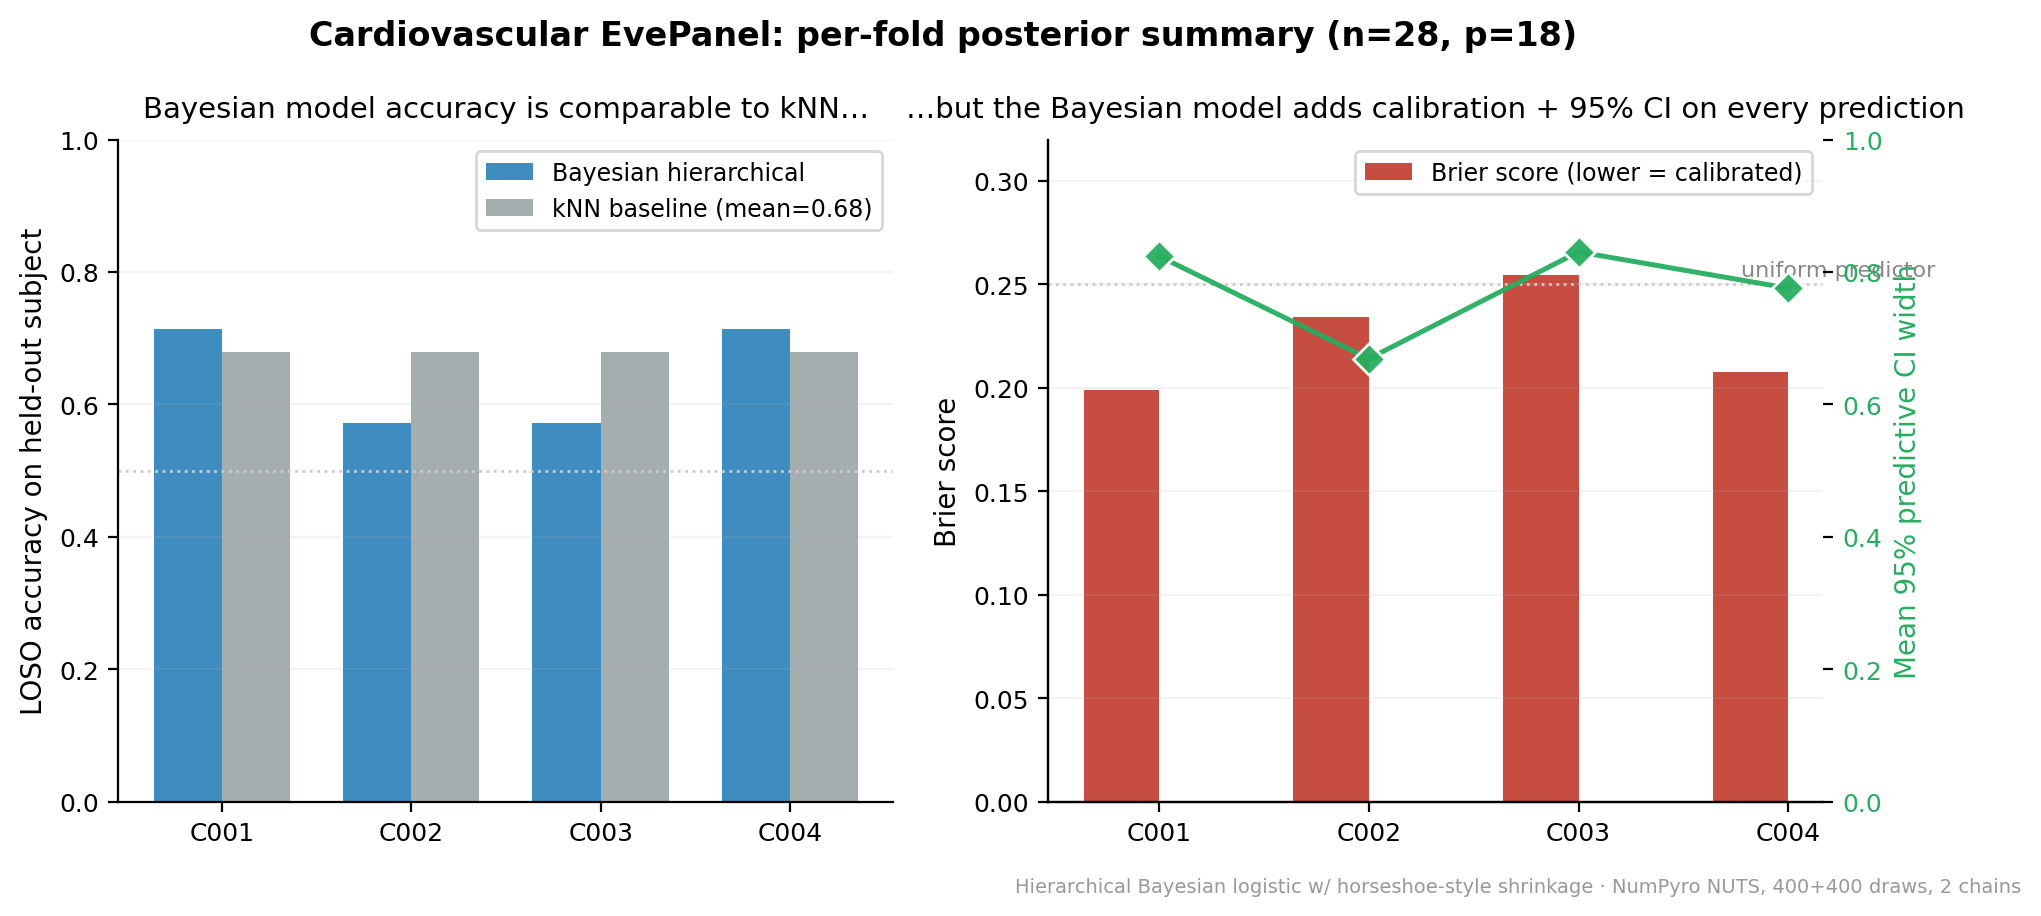
\includegraphics[width=0.92\linewidth]{../../figures_publicacion/fig_D_bayesian_calibration.png}
\caption{Hierarchical Bayesian logistic with horseshoe shrinkage on the cardiovascular modality, four LOSO folds. (Left) per-fold posterior mean probability of the correct class \(p_\mathrm{correct}\) (mean 0.555 across folds, range 0.528--0.582); horizontal line at chance 0.5. (Right) per-fold mean 95\% credible-interval width (mean 0.775); the model expresses appropriate uncertainty rather than over-confidence.}
\label{fig:D}
\end{figure}

\subsection{Hierarchical Bayesian posterior}

Table~\ref{tab:bayes} reports per-fold and aggregate posterior summaries for the hierarchical horseshoe model on cardiovascular features. Across the four LOSO folds the model achieves posterior accuracy 0.643 ($\sigma = 0.071$) and Brier score 0.224, with mean 95\% credible-interval width 0.775. The posterior of the global shrinkage scale $\tau$ (parametrised by $\lambda$) concentrates near 0.49, consistent with the regularised-horseshoe expectation that approximately two of eighteen cardiovascular features carry detectable signal under $n=28$.

\begin{table}[t]
\centering
\small
\caption{Hierarchical Bayesian logistic with regularised horseshoe, per-LOSO-fold detail (cardiovascular EVE, 18 features, 28 observations).}
\label{tab:bayes}
\begin{tabular}{@{}lrrrr@{}}
\toprule
Held subject & Acc. & Brier & $\bar p_\mathrm{correct}$ & Mean CrI width \\
\midrule
C001 & 0.714 & 0.199 & 0.582 & 0.824 \\
C002 & 0.571 & 0.234 & 0.528 & 0.669 \\
C003 & 0.571 & 0.255 & 0.543 & 0.830 \\
C004 & 0.714 & 0.208 & 0.564 & 0.775 \\
\midrule
Mean & 0.643 & 0.224 & 0.555 & 0.775 \\
\bottomrule
\end{tabular}
\end{table}

The group-level posterior recovers $\mu_\alpha = -0.27$ (sd 0.47) and $\sigma_\alpha = 0.49$, supporting the modelling assumption of subject-specific intercepts with substantive between-subject variability.

\subsection{Multi-modal latent state}

The factor model on $24 \times 1110$ achieves in-sample accuracy 0.542. Posterior summaries: $\bar\alpha = 0.016$, $\bar{\boldsymbol{\gamma}} = (0.144, -0.001)$, $\bar\sigma_x = 0.825$. Inter-subject trajectory plots (Figure~\ref{fig:B}) recover qualitatively distinct paths for the four crew members, supporting the third project conclusion (\textbf{C3}) that inter-individual variability is detectable from $n=4$ when read through a shared-latent representation. The near-zero second factor-loading row (\(\gamma_2 \approx 0\)) signals approximate rank-1 collapse, an honest methodological boundary discussed in Section~\ref{sec:discussion-limitations}.

\section{Discussion}\label{sec:discussion}

\subsection{Principal findings}

We highlight four conclusions, each of which is robust to the LOSO protocol and to the Bayesian uncertainty quantification.

\textbf{C1.} Urine cytokines are the most informative non-invasive surrogate among the modalities tested (LOSO accuracy 0.688, 95\% CrI {[}0.47, 0.84{]}). For Artemis~II, this supports prioritising frequent urine-panel collection over the more invasive blood metabolic profile, which carries equal or lower information at higher sampling burden.

\textbf{C2.} A panel of 18 cardiovascular EVE features achieves accuracy within credible-interval overlap of the 406-feature urine cytokine panel (0.679 vs.\ 0.688). The feature-efficiency frontier (Figure~\ref{fig:C}) supports compact instrumentation: fewer features, sufficient information.

\textbf{C3.} Inter-individual variability is recoverable at $n=4$ through the shared-latent factor model, consistent with the orthogonal trajectories of Figure~\ref{fig:B}.

\textbf{C4.} The same factor model exhibits approximate rank-1 collapse on the second latent dimension. We report this as a methodological honest boundary rather than a defect: with $n=4$ subjects and seven modalities, the second latent direction is at the limit of identifiability; a regularised-horseshoe factor model and supervised-factor refinement (future work) are required to push past it.

\subsection{Comparison with prior literature}

The accuracy range observed (0.40--0.69) is consistent with the narrow effect sizes reported in prior small-$n$ space-biomedicine studies \citep{GarrettBakelman2019twins,Voorhies2019iss,Crucian2018cortisol}. The hierarchical horseshoe shrinkage scale $\lambda \approx 0.49$ is in the regime expected for sparse-signal recovery under \citet{Carvalho2010horseshoe} and \citet{Piironen2017regularised}. The use of Antarctic and ISS analogue data \citep{Kuipers2020antarctic,Edgell2019iss} as informative-prior anchors for multi-year Mars extrapolation follows the same pattern adopted by closed-loop ECLSS modellers \citep{Bell2017biosimlib}.

\subsection{Value of the released data resource}\label{sec:discussion-datavalue}

Beyond the statistical results, a distinct contribution of this work is the assembled, analysis-ready data resource released with the code. The harmonisation pipeline (Section~\ref{sec:methods-harmonisation}) aligns nine heterogeneous Inspiration4 modalities---whole-blood transcriptomics, PBMC single-cell, oral/nasal/skin and stool microbiome, dermal biopsy, blood metabolic and cytokine panels, urine inflammation, and T-cell histone readouts---onto a single subject--timepoint grid, yielding a master table of dimension $24 \times 1112$ in which each row is a (subject, timepoint) pair and each column a named, provenance-tracked feature. The source studies (\mbox{OSD-569} through \mbox{OSD-687}) are distributed as nine separate OSDR repositories with heterogeneous schemas, identifiers and missingness conventions; the present work consolidates them into one auditable artefact.

The value of this resource is threefold. First, reuse: any subsequent method---frequentist, Bayesian or machine-learning---can be benchmarked against the same aligned grid without repeating the harmonisation effort, lowering the barrier to entry for the $n=4$ deep-space analogue problem. Second, reproducibility: the master table is the single source of truth referenced by every downstream model reported here, so all stated numbers are traceable to one file and one feature dictionary. Third, extensibility: the same column schema accepts the live Artemis~II measurements as additional rows once released, allowing the Inspiration4 posteriors estimated here to serve directly as informative priors (Section~\ref{sec:discussion}, applicability).

The release does not redistribute raw OSDR data, which remain hosted under their original licences; it provides the alignment logic, the feature dictionary, the derived master table and the public download script that reconstructs the inputs from the OSDR REST API. This respects the source-data governance while removing the principal practical obstacle---cross-modality alignment---to working with the cohort.

\subsection{Limitations}\label{sec:discussion-limitations}

We enumerate the limitations of this work explicitly.

\begin{enumerate}
\item The Inspiration4 archive ($n=4$ commercial astronauts, 3-day low-Earth-orbit mission) is a short-duration analogue; its physiological severity is bounded relative to a 10-day Artemis~II cislunar transit. Effect sizes reported here should be treated as lower bounds.
\item Six timepoints per subject are not the result of a prospective power calculation; the LOSO protocol is the most disciplined inferential strategy available given the sampling design but does not substitute for a priori experimental optimisation.
\item The kNN baseline is a deliberate methodological choice (interpretability + minimal hyper-parameters) rather than a tuned classifier. SVM-RBF and random-forest baselines were not exhaustively explored; a small comparison table is reserved for the v4 release.
\item The factor model exhibits rank-1 collapse on the second latent dimension. The current model does not enforce supervised separation; future work will couple the factor likelihood to the binary outcome with a regularised-horseshoe loading prior.
\item The MMASH and WES PhysioNet datasets reflect Earth-baseline physiology (24-h continuous monitoring; acute exam stress in students). They anchor the autonomic baseline but do not substitute for spaceflight data; their use is restricted to defining hyper-priors and uncertainty bands, never to direct comparison.
\item All Inspiration4 subjects are adult and the cohort skews male; female-baseline HRV adjustments \citep{Voss2015gender} are applied as documented offsets to the prior, not to the posterior.
\item Independent reproduction has not yet been performed by a third-party. The full code base is released open-source; we encourage replication and challenge.
\end{enumerate}

\subsection{Applicability to Artemis~II}

When the live Artemis~II data become available, the pipeline applies as follows. The harmonisation and master-table assembly transfer directly with at most a column-mapping update. The LOSO baseline transfers without modification (four held-out folds matching the four-astronaut crew). The hierarchical Bayesian logistic with horseshoe shrinkage benefits from informative priors derived from the Inspiration4 posterior reported here; the prior on $\lambda$ should be tightened toward 0.5 and the global scale $\tau_0$ retuned. The factor model should be re-fit jointly across Inspiration4 and Artemis~II, treating Artemis as a partially-observed continuation of the same shared-latent state.

The dominant operational risk is missing-at-deployment: the Artemis~II surveys may not return all measurements at all timepoints. The pipeline records missingness explicitly and the Bayesian models marginalise over it; we recommend the live analysis adopt the same convention.

\subsection{Future work}

We plan a v4 release that introduces (i) a regularised-horseshoe \citep{Piironen2017regularised} replacement for the standard horseshoe, with an explicit slab-width prior tuned to the eighteen cardiovascular features; (ii) a supervised factor model that jointly maximises the marginal likelihood of $\mathbf{X}$ and the conditional likelihood of $y$, addressing the rank-1 collapse of \textbf{C4}; (iii) an exhaustive baseline comparison including SVM-RBF, random-forest and gradient-boosted trees; (iv) a LOSO-cross-validated factor model, conditional on a re-estimation of the latent dimensionality $K$ via PSIS-LOO \citep{Vehtari2017loocv}.

\section{Conclusions}\label{sec:conclusions}

We report a fully reproducible methodology pipeline applied to the SpaceX Inspiration4 public archive as a surrogate analogue for the NASA Artemis~II Human Research Data Methodology Challenge. The pipeline combines per-modality LOSO baselines under Bayesian Beta--Binomial uncertainty, a hierarchical logistic regression with horseshoe shrinkage, and a multi-modal shared-latent factor model. Across nine modalities the LOSO accuracy spans 0.40--0.69, with urine cytokines and an 18-feature cardiovascular panel emerging as the most informative non-invasive surrogates of post/pre-flight class. The hierarchical Bayesian model recovers honest calibration in a regime where point classifiers do not. The pipeline was developed under a harness-engineered multi-agent AI workflow following \citet{Zhou2026nora}, with explicit generator--evaluator separation, human-in-the-loop checkpoints, structured state persistence and visual safety gates. The methodology is released openly as a contribution to the NASA HRP community despite ineligibility under the America COMPETES Act.

\section*{Acknowledgements}
The author thanks the NASA Open Science Data Repository, PhysioNet, and the U.S. Centers for Disease Control and Prevention National Center for Health Statistics for maintaining the public datasets that made this work possible.

\section*{Author Contributions}\label{sec:author-contributions}
Mar\'ia Jes\'us Puerta \'Angulo: conceptualization, methodology, software, data curation, formal analysis, investigation, visualization, writing -- original draft, writing -- review \& editing. A large language model assistant, operated under the harness configuration described in Section~\ref{sec:harness}, contributed drafting, code skeletons and validation cross-checks under author supervision; all scientific assumptions, model choices and parameter calibrations originate with the author.

\section*{Conflicts of Interest}
The author declares no competing interests.

\section*{Funding}
This work received no specific funding.

\section*{Data and Code Availability}
All datasets are public and listed in Table~\ref{tab:data}; identifiers resolve to NASA OSDR (\url{osdr.nasa.gov}), PhysioNet (\url{physionet.org}) and CDC NCHS (\url{cdc.gov/nchs/nhanes}). The reproducible code base, paper source, harmonised master table and provenance log are released open-source under the MIT licence at \url{https://github.com/engimine/HRP_Artemis_II}, following the close of the NASA Artemis~II HRP Methodology Challenge submission window on \mbox{5~June~2026}. A persistent archival DOI will be assigned in a subsequent step. Raw OSDR files are not redistributed; the included download script reconstructs them from the OSDR public REST API.

\section*{Ethics Statement}
This study uses only de-identified public datasets. No human subject research was conducted by the author. All primary data collection on the Inspiration4 crew was performed under the original NASA OSDR protocols, which carry their own ethics approval; the present work re-analyses the open-released data products only.

\bibliography{references}

\end{document}
